\begin{figure}
  \centering
  Model. A
  \begin{tabular}{ccc}
    \begin{minipage}{0.330\hsize}
      \centering
      $\pi^-\Sigma^+$ mode
      \includegraphics[width=4.5cm]{../pic/discussion/pimSp_A.eps}
    \end{minipage}
    
    \begin{minipage}{0.33\hsize}
      \centering
      $\pi^+\Sigma^-$ mode
      \includegraphics[width=4.5cm]{../pic/discussion/pipSm_A.eps}
    \end{minipage}
    
    \begin{minipage}{0.33\hsize}
      \centering
      $\pi^0\Sigma^-$ mode
      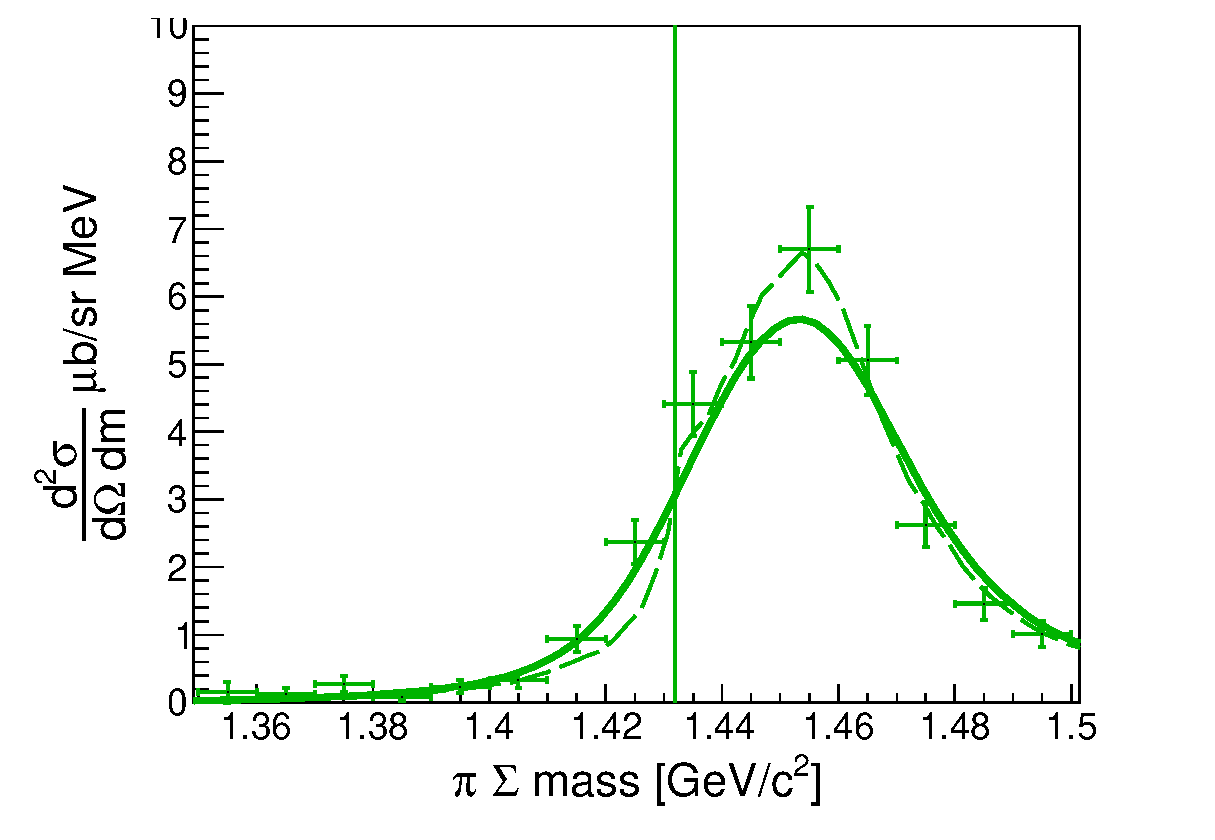
\includegraphics[width=4.5cm]{../pic/discussion/pimS0_A.eps}
    \end{minipage}
  \end{tabular}
  Model. B
  \begin{tabular}{ccc}
    \begin{minipage}{0.33\hsize}
      \centering
      $\pi^-\Sigma^+$ mode
      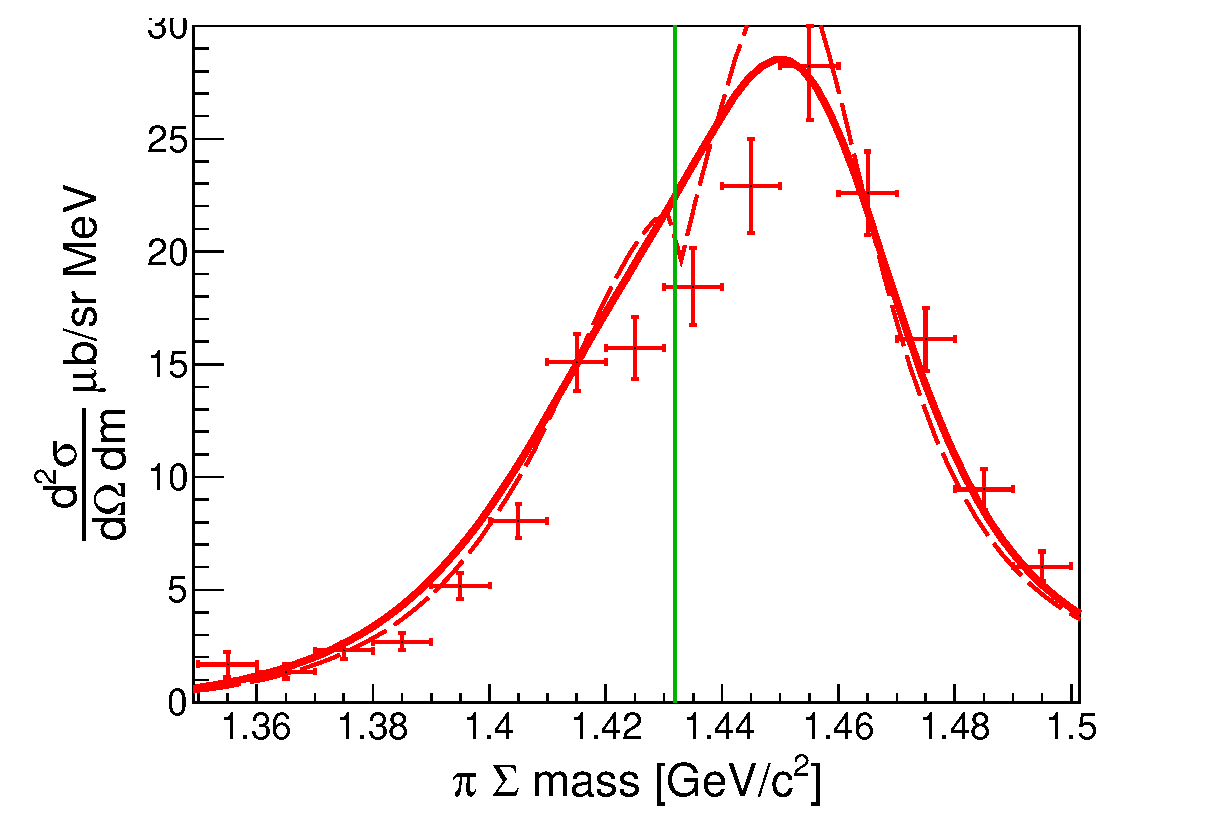
\includegraphics[width=4.5cm]{../pic/discussion/pimSp_B.eps}
    \end{minipage}
    
    \begin{minipage}{0.33\hsize}
      \centering
      $\pi^+\Sigma^-$ mode
      \includegraphics[width=4.5cm]{../pic/discussion/pipSm_B.eps}
    \end{minipage}

    \begin{minipage}{0.33\hsize}
      \centering
      $\pi^0\Sigma^-$ mode
      \includegraphics[width=4.5cm]{../pic/discussion/pimS0_B.eps}
    \end{minipage}
  \end{tabular}
  \caption{
    This figures shows obtained spectra and DCC calculation \cite{DCC2}.
    Error bar indicates obtained spectra.
    Dashed and solid line indicate theoretical calculation itself and calculation convoluted by detector resolution, respectively.
    Left, center and right figures represent \pimSp, \pipSm and \pimSz, respectively.
  }
  \label{fig:compDCC}
\end{figure}
